\documentclass{article}
\usepackage[left=1in, right=1in, top=1in, bottom=1in]{geometry}
\usepackage{mathexam}
\usepackage{amsmath}
\usepackage{graphicx,subcaption}
\usepackage{booktabs}
\usepackage{enumitem}
\usepackage{atbegshi}% http://ctan.org/pkg/atbegshi
\usepackage[ruled,linesnumbered]{algorithm2e}
\AtBeginDocument{\AtBeginShipoutNext{\AtBeginShipoutDiscard}}

%\ExamClass{Sample Class}
%\ExamName{Sample Exam}
%\ExamHead{\today}

%\let\ds\displaystyle

\begin{document}

\begin{titlepage}
	\vspace*{\stretch{1.0}}
	\begin{center}
		\Large\textbf{Rectifying Bound}\\
		\large\textit{20 September 2018}
	\end{center}
	\vspace*{\stretch{2.0}}
\end{titlepage}














\section{Rectifying wrong upper bound on Adaptive Pruning schemes}


In order to reduce costs, our DiVE schemes utilize the importance score bound to do pruning. There are two pruning techniques proposed: 1) static bound approach and 2) adaptive bound approach. In static bound, the theoritical upper bound ($ \sqrt{2} $) is used and this bound will not be changed until the end of iteration. Meanwhile, adaptive scheme estimates upper bound based on view queries that have been executed, the bound is updated where there is a higher upper bound found on the next query execution. 


In order to know how many samples that need to be executed to estimate the upper bound, samping based on prediction interval is used. Before running the scheme, user needs to define what PI that she wants to use. For instance, while user uses PI 80, it means the current bound will be updated to the maximum importance score which have seen so far of 9 executed views. Generally, PI can be defined as following: 

%In the algorithm \ref{DiVE-Greedy-Pruning-Rectifying} and \ref{DiVE-dSwap-Pruning-Rectifying}, $getMaxPI(L)$ is the function to get the estimated upper bound from some number of executed views based on PI. 

\begin{itemize}[noitemsep]
	\item PI80: need to execute 9 sample of views
	\item PI85: need to execute 12 sample of views
	\item PI90: need to executes 20 sample of views
	\item PI95: need to executes 40 sample of views
	\item PI97: need to executes 60 sample of views
\end{itemize}

\begin{figure}
	\begin{center}
		\vspace{-15pt}
		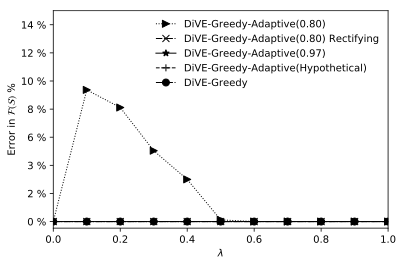
\includegraphics[width=3.0in]{figures/rectifiying_error_f_s_greedy}
		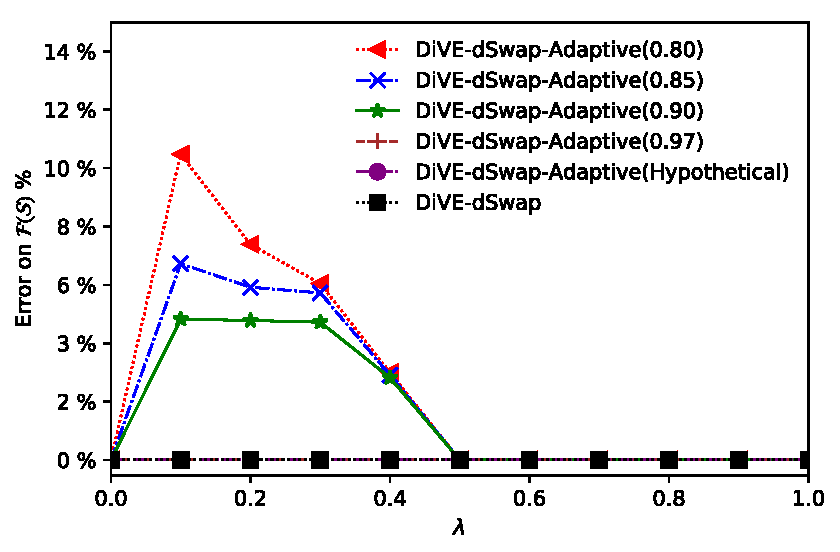
\includegraphics[width=3.0in]{figures/rectifiying_error_f_s_dswap}
		\caption{Error $F(S)$ Adaptive Pruning}
		\label{fig:error_fs_adaptive}
	\end{center}
\end{figure}

Our experiment results show that Adaptive scheme has the best pruning performance while PI80 is used. However, it reduces the effectiveness of recommended views due to only small number of sample executed views are needed that leads to wrong estimation of upper bound. Figure \ref{fig:error_fs_adaptive} shows the error in $F(S)$ in different value of $PI$. The safest way is to use higher PI such as PI95 or PI97 but it needs to execute more views which contradict to our propose to minimizing the cost.  

If there is a way to use PI80 without reducing effectiveness, it will definitely very good. In fact, \textit{the goal of our pruning scheme is to minimize query view execution (i.e., use low $PI$) without reducing the quality of recommended views}. In order to overcome this issue, rectifying bound of adaptive pruning is proposed. The algorithms of our rectifying bound can be seen in algorithm \ref{DiVE-Greedy-Pruning-Rectifying} for DiVE-Greedy-Adaptive and \ref{DiVE-dSwap-Pruning-Rectifying} for DiVE-dSwap-Adaptive. The detail our rectifying technique is presented below:


\begin{figure}
	\centering
	\begin{minipage}{0.45\textwidth}
		\centering
		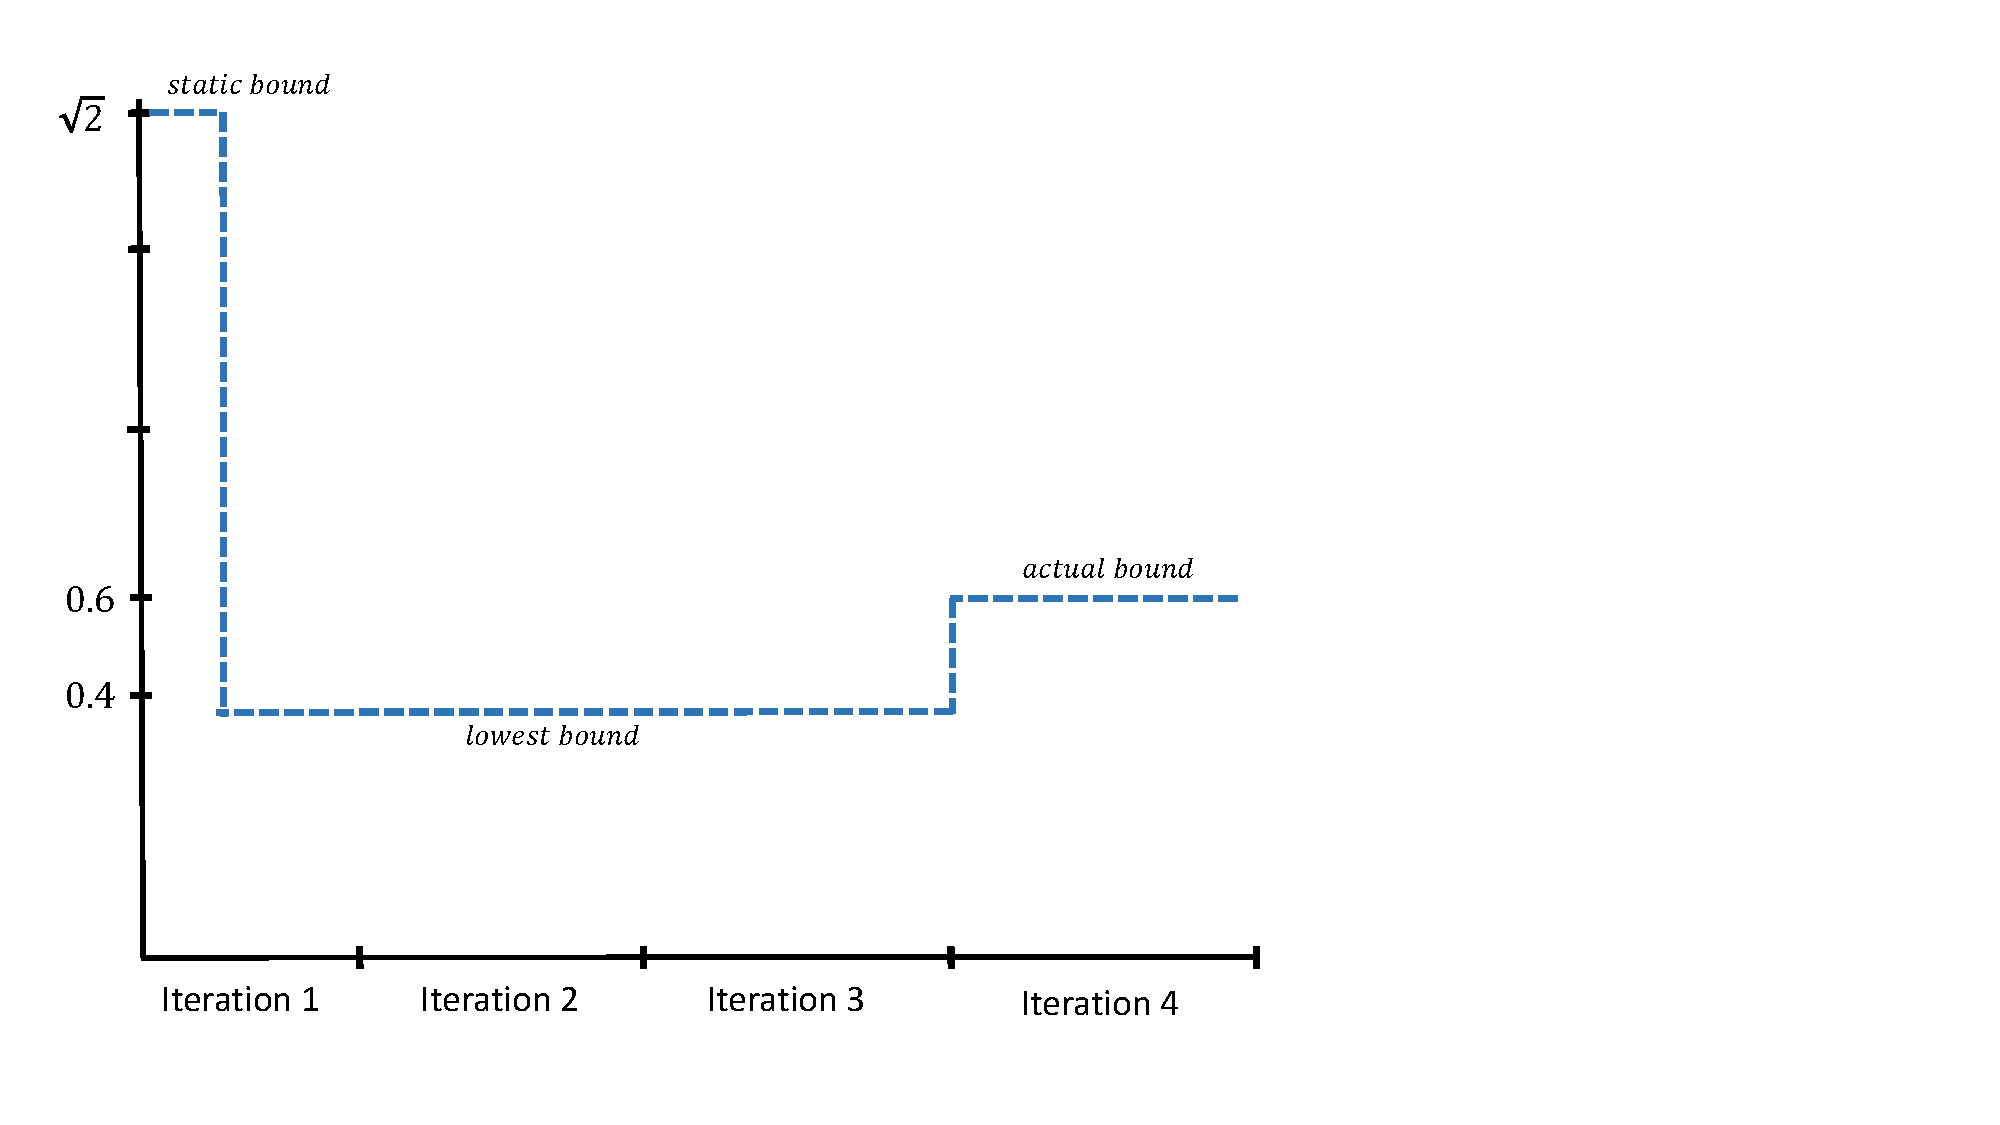
\includegraphics[width=1.5\textwidth]{figures/Rectifying_flow_graph} % first figure itself
		\caption{The changing of upper bound in each iteration of DiVE-Greedy-Adaptive}
		\label{fig:rectify_logic_graph}
	\end{minipage}\hfill
	\begin{minipage}{0.45\textwidth}
		\centering
		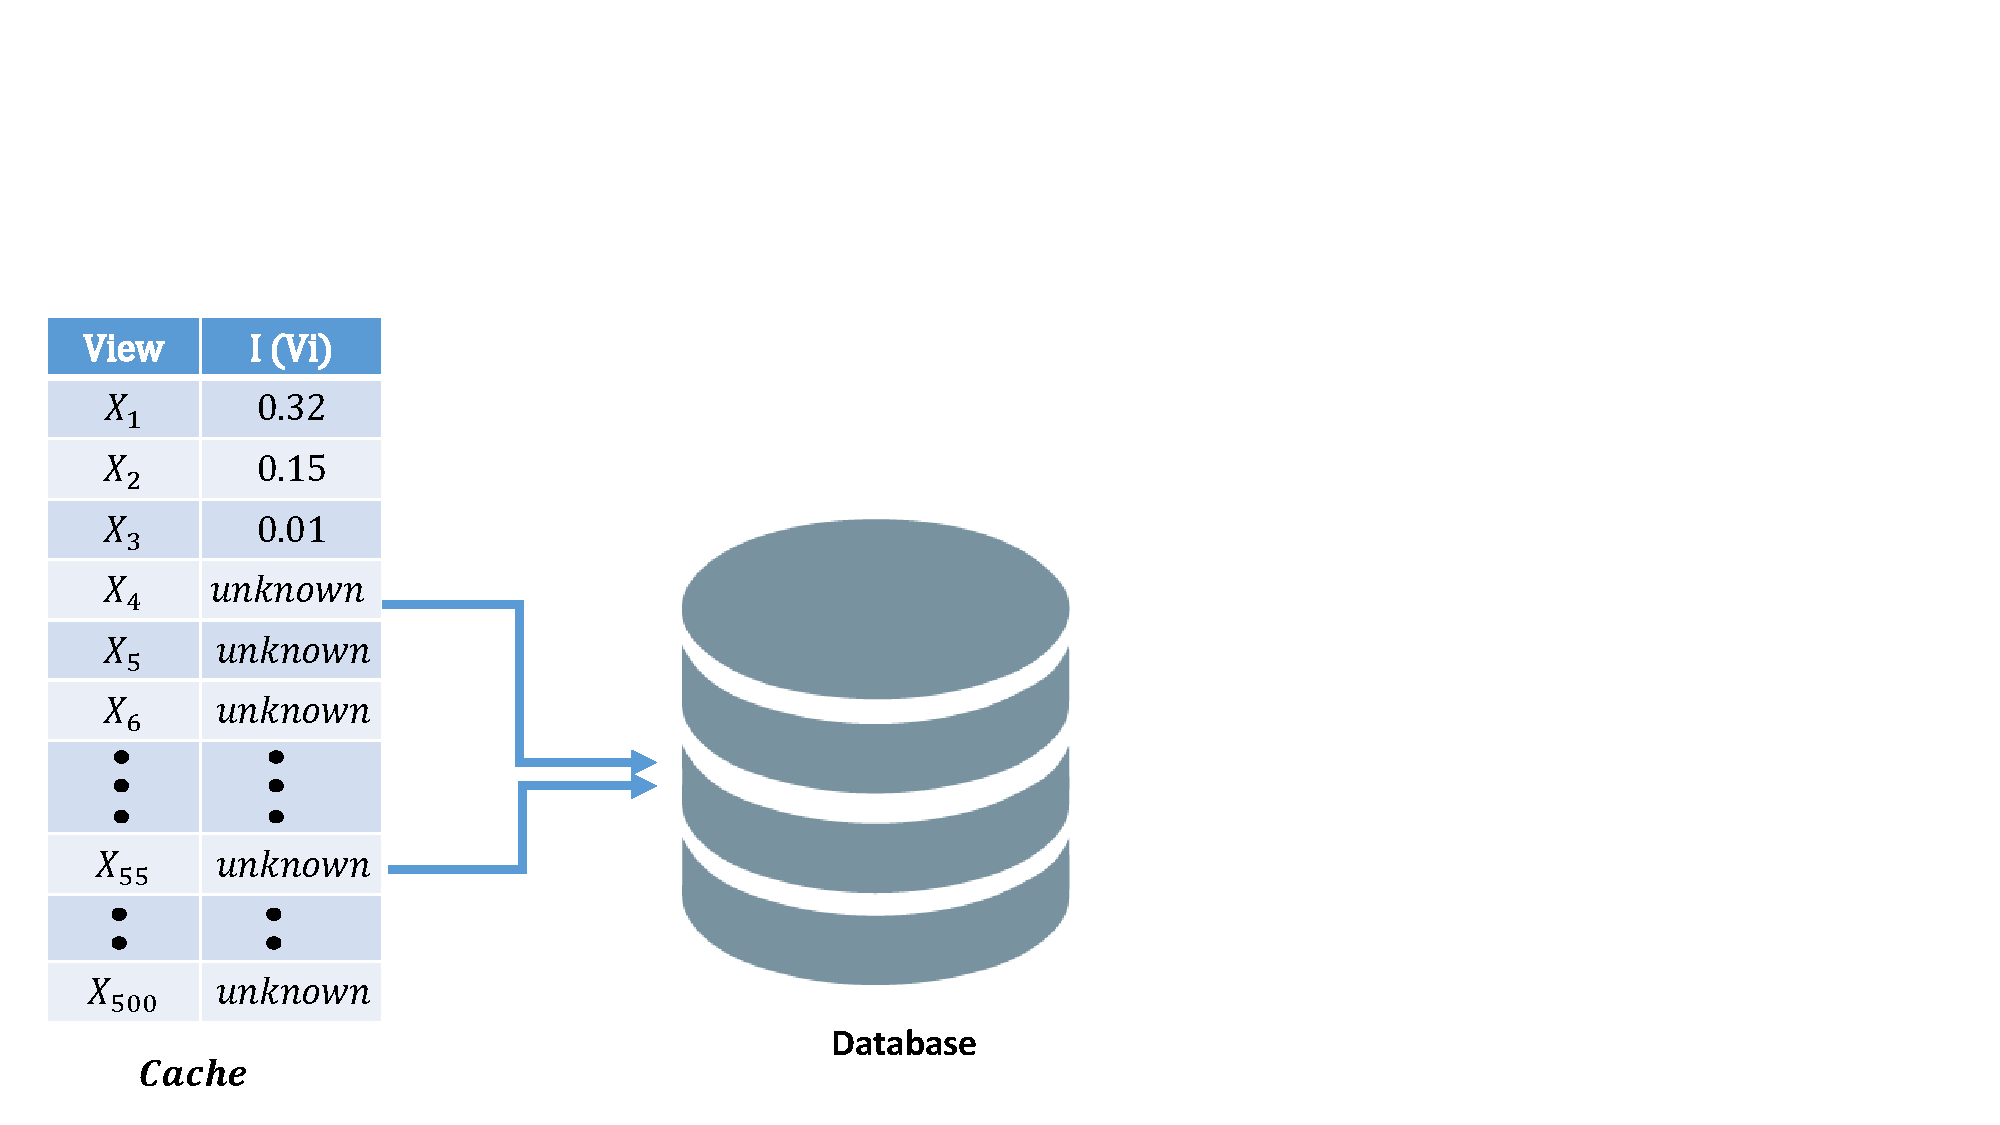
\includegraphics[width=1.5\textwidth]{figures/cache} % second figure itself
		\caption{Caching storage of query execution}
		\label{fig:cache}
	\end{minipage}
	
\end{figure}



\subsection{Rectifying upper bound}
As mentioned above that static pruning uses theoritical upper bound $(\sqrt{2})$ until the end of iteration and there is no mechanism to update the bound. Hence, the pruning performance is not working optimal due to the theoritical upper bound may very far from the actual upper bound from the dataset (e.g., the actual bound = 0.6). To overcome this issue, adaptive pruning is proposed to estimate the upper bound by executing some sample of views and the upper bound will be updated while in the next execution the higher bound is found. However, adaptive pruning leads to over-prune due to the estimated upper bound may far below the actual bound (e.g., actual bound = 0.6, estimated bound = 0.3). Consequently, it reduces the quality of the recommended views or produces error in $F(S)$. Without rectifying upper bound, the error in $F(S)$ in different value of $PI$ can be seen in Figure \ref{fig:error_fs_adaptive}.

In order to eliminate error in $F(S)$ and keep the high pruning performance, rectifying upper bound is proposed. The idea behind the rectifying bound technique is to support backtracking. For instance, Figure \ref{fig:rectify_logic_graph} shows the changing of upper bound in each iteration of DiVE-Greedy-Adaptive. Let assume that user defines $k = 6$, as size of the initialization of set $S$ equal to 2, there will be four times iterations to recommend set $S$ which $k = 6$. Similar to the static pruning approach, as the initialization, $(\sqrt{2})$ is used as the upper bound. The scheme runs with the upper bound is equal to $(\sqrt{2})$ in the first iteration. While certain number sample of views are executed and have been fullfilled the $PI$ condition (e.g., PI80 needs 9 samples of executed views), the upper bound will be updated to the maximum importance score of views have seen so far (e.g., 0.4). As shown in Figure \ref{fig:rectify_logic_graph} there are no importance score of executed views in the first, second, and third iteration that higher than the current upper bound (0.4). However, in the last iteration (iteration 4), the higher bound is found (e.g., 0.6). In this example, it shows that in the second and third iteration, the scheme runs with wrong upper bound which may leads to over-prune and reduce the effectiveness. Without rectifying, the result are presented to users as the final result. Meanwhile, with rectifying strategy the backtracking is supported. The scheme is able to backtrack to the first iteration and uses the correct upper bound for the next iterations. 

In the next section, we explain the detail of our rectifying strategy that consists of two important techniques: 1) Bookkeeping (keep tracking the result in each iteration) and 2) Caching (utilize cache to optimize re-using strategy).

\subsubsection{Bookkeeping Technique}
In order to support rectifying bound, bookkeeping technique is used. The idea behind this technique is to keep track: 1) the set $S$ as the input in each iteration and 2) list $L$ in each iteration and 3) the position of maximum $setDist$ score in $L$ while it gets early termination. For instance, Figure \ref{fig:rectify_logic_column} shows the rectifying algorithm of DiVE-Greedy-Adaptive while $k = 6$. Firstly, there are two most distant views in the set $S$ as the initialization and $\sqrt{2}$ as the upper bound. In each iteration, Greedy add one most optimal view to the set $S$, the iteration will stop while $k = 6$. The detail of bookkeeping technique in our rectifying strategy as follows.

A list $L$ of all views in $X$ is created such that each $X_i$ is assigned an importance equal to the upper bound $I_u$ and $L$ is sorted based on the diversity score of each view $X_i$ to the current set $S$ as shown in Figure \ref{fig:rectify_logic_column}.
The goal for DiVE-Greedy is to find the view with the highest utility $U(H)$. As described in %Eq. ~\ref{utility_each_candidate} 
utility function equation, such utility score $U(X_i)$ is a weighted sum of two measures: 1) the importance score of $X_i$ (i.e., $I(X_i)$), and 2) the distance of $X_i$ from $S$ (i.e., $ setDist\left(X_i, S\right)$). Then, the highest utility $U(H)$ is initialized to a default value of 0.0, and the list $L$ is traversed in order. 
%
For each visited view $X_i$, the upper bound on the utility achieved by $X_i$ (i.e., $maxU(X_i)$) is computed using its actual diversity score and the upper bound on its importance.
%
If $maxU(X_i) > U(H)$, then $X_i$ is generated and its actual utility $U(X_i)$ is calculated. 
%
Accordingly, if $U(X_i) > U(H)$, then $U(H)$ is set to be equal to $U(X_i)$. 
%
However, if $maxU(X_i) < U(H)$, then early termination is reached. 

\begin{figure}
	\begin{center}
		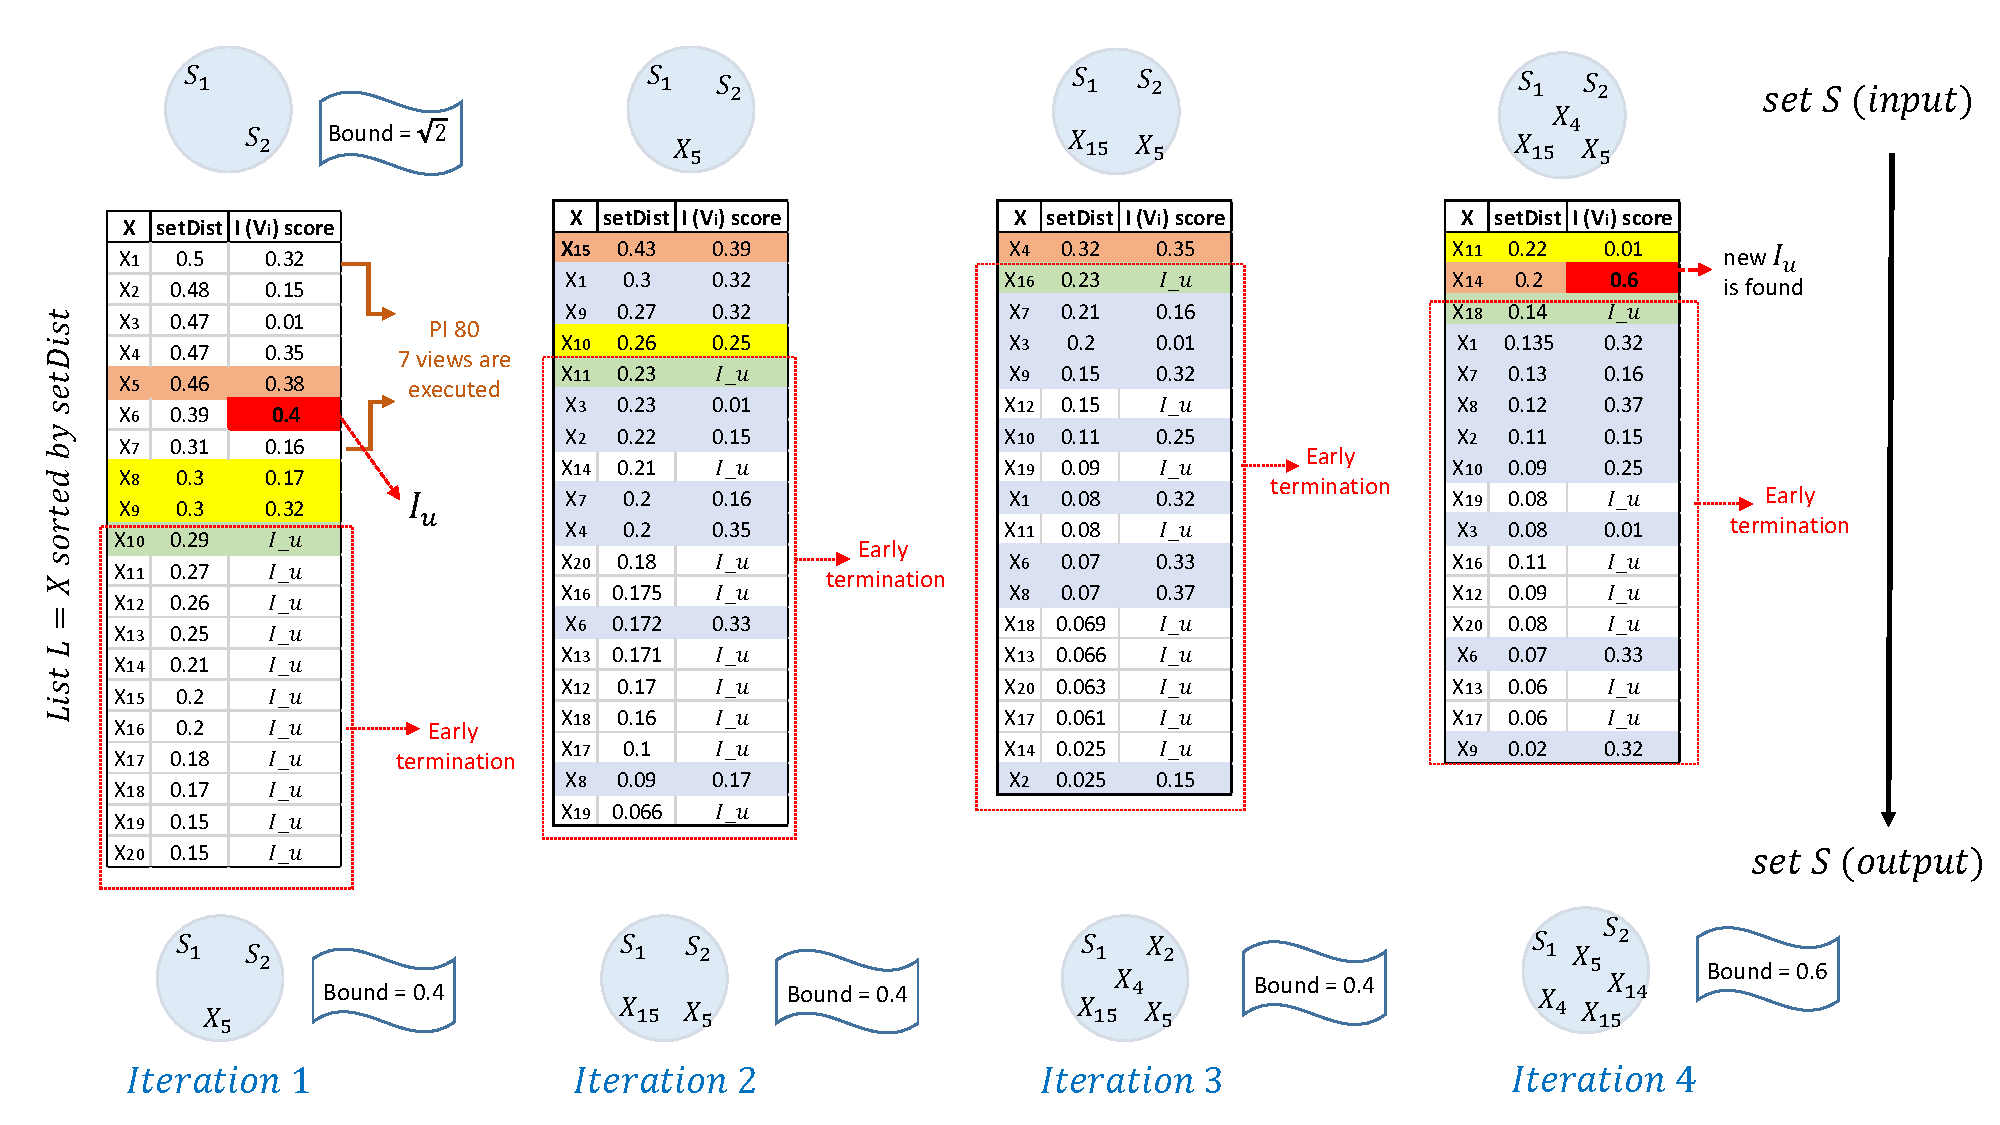
\includegraphics[width=7.0in]{figures/Rectifying_flow_column}
		\vspace{-8pt}
		\caption{Rectifying upper bound in DiVE-Greedy-Adaptive while $k = 6$}
		\label{fig:rectify_logic_column}
		
	\end{center}
\end{figure}
Let start from the first iteration, for instance, $PI80$ is used which needs 9 sample executed views. There are two views in set $S$, it needs 7 more views to be executed to update the upper bound $I_u$ as shown in Figure \ref{fig:rectify_logic_column} (e.g., $V_1 - V_7$ in Iteration 1). Let assume that from the executed views, 0.4 is the higest importance score, then $I_u$ is updated from $\sqrt{2}$ to 0.4. After $I_u$ is updated to 0.4, early termination is reached on $V_{10}$. Hence, $V_{10}$ and all views below of $V_{10}$ can be ignored. Meanwhile, all views above $V_{10}$ (e.g., $V_8, V_9$) need to be executed because these views satisfy the condition $maxU(X_i) > U(H)$. As shown in this Figure, the highest importance score of all executed views still 0.4 and there are no more views in Iteration 1 that need to be executed. Finally, view with the highest utility $U(H)$ is added to set $S$ (e.g., $V_5$). 

In the next iteration, the size of set $S$ is increased because one view is added in each iteration. A new list $L$ is created and $setDist$ score is recalculated. Similar to the first iteration, list $L$ is sorted based on $setDist$ score. 
Figure \ref{fig:rectify_logic_column} shows that in the second and third iterations, there are no importance score of executed views that higher than 0.4. Hence, there is no updating the upper bound in the second and third iterations. However, the higher upper bound is found in forth iteration (e.g., 0.6). In this condition, we realize that the scheme used wrong upper bound in the previous iterations that may lead to over-prune and reduce the quality of recommended views. 

In order to fix the wrong bound in the previous iterations, bookkeeping startegy is used in this approach. In each iteration, list $L$, set $S$ ($S$ as the input), and view which early termination is started (e.g., $V_{10}, V_{11}, V_{16}, V_{18}$ in Iteration 1,2,3,4 respectively) are stored. The position of view when early termination started is important because it needs to be evaluated using the correct upper bound. 

According to the example in Figure \ref{fig:rectify_logic_column}, the higher upper bound is found in the forth iteration. Hence, upper bound which used in the previous iterations is wrong. In order to fix it, the scheme is able to go back and start from the previous iteration using $L$ and $S$ of the previous iteration which are stored before. This bookeeping technique can be seen in Algorithm \ref{DiVE-Greedy-Pruning-Rectifying} for DiVE-Greedy-Adaptive (e.g., line 30 - 34) and \ref{DiVE-dSwap-Pruning-Rectifying} (e.g., line 32 - 37) for DiVE-dSwap-Adaptive.

Rectifying bound needs forward and backward looping that may leads to higher costs. To overcome this issue, we propose Caching mechanism which can reduce the cost by reusing strategy as presented in the next section. 

\subsubsection{Caching Technique}
The results of this rectifying bound strategy can be seen in Figure \ref{fig:rectifying_bound}. The results are average from five queries. These Figures show the performance of adaptive pruning scheme with rectifying bound strategy compared to without rectifying bound strategy. The pruning peformance after applying rectifying bound strategy quite close to without rectifying bound strategy. Meanwhile, as shown in Figure \ref{fig:error_fs_rectifying} there is no effectiveness loss after rectifying bound is implemented especially for PI80. Moreover, the costs comparison of our rectifying algorithm is also presented in Figure \ref{fig:flight_costs_all_rectifying}. This Figure shows the total cost of our pruning scheme with and without rectifying bound strategy which running on Flights dataset. 

The results of this rectifying bound strategy can be seen in Figure \ref{fig:rectifying_bound}. The results are average from five queries. These Figures show the performance of adaptive pruning scheme with rectifying bound strategy compared to without rectifying bound strategy. The pruning peformance after applying rectifying bound strategy quite close to without rectifying bound strategy. Meanwhile, as shown in Figure \ref{fig:error_fs_rectifying} there is no effectiveness loss after rectifying bound is implemented especially for PI80. Moreover, the costs comparison of our rectifying algorithm is also presented in Figure \ref{fig:flight_costs_all_rectifying}. This Figure shows the total cost of our pruning scheme with and without rectifying bound strategy which running on Flights dataset. 

\section{Experiment Results}
The results of this rectifying bound strategy can be seen in Figure \ref{fig:rectifying_bound}. The results are average from five queries. These Figures show the performance of adaptive pruning scheme with rectifying bound strategy compared to without rectifying bound strategy. The pruning peformance after applying rectifying bound strategy quite close to without rectifying bound strategy. Meanwhile, as shown in Figure \ref{fig:error_fs_rectifying} there is no effectiveness loss after rectifying bound is implemented especially for PI80. Moreover, the costs comparison of our rectifying algorithm is also presented in Figure \ref{fig:flight_costs_all_rectifying}. This Figure shows the total cost of our pruning scheme with and without rectifying bound strategy which running on Flights dataset. 





\begin{figure}
	\begin{center}
		%\vspace{-20pt}
		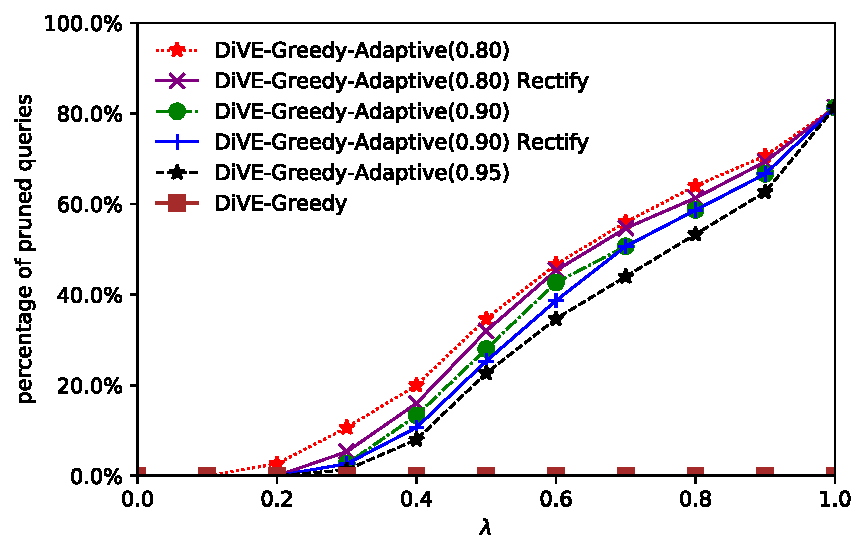
\includegraphics[width=3.0in]{figures/pruning_performance_greedy_adaptive_rectifying_compare}
		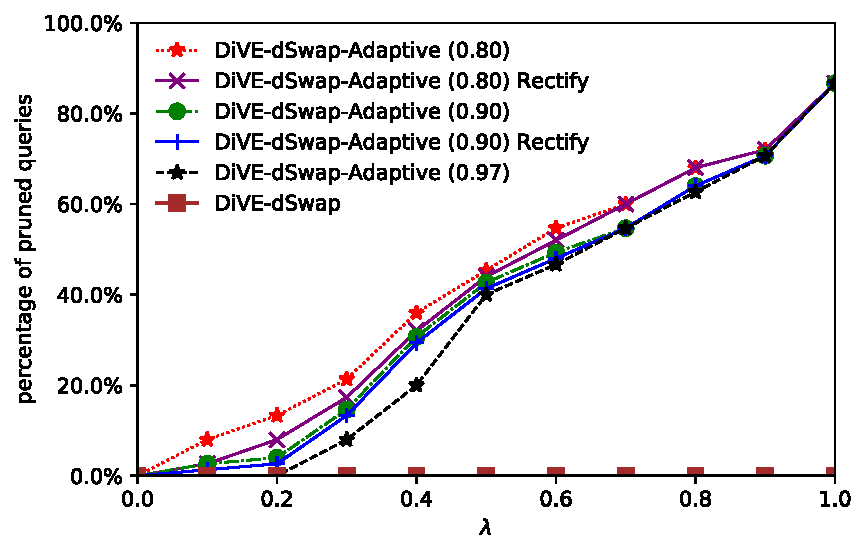
\includegraphics[width=3.0in]{figures/pruning_performance_dswap_adaptive_rectifying_compare}
		\caption{Rectifying bound DiVE-Greedy-Adaptive and DiVE-dSwap-Adaptive}
		\label{fig:rectifying_bound}
	\end{center}
\end{figure}

\begin{figure}
	\begin{center}
		%\vspace{-20pt}
		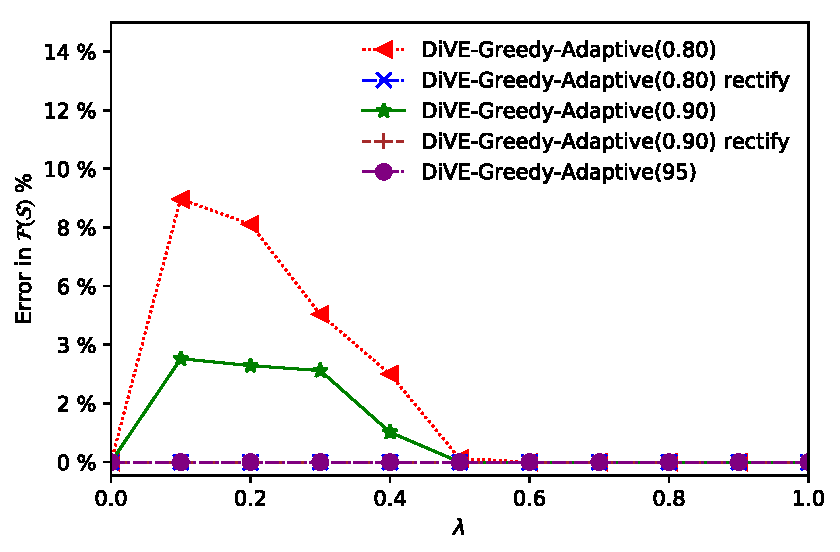
\includegraphics[width=3.0in]{figures/error_fs_rectifying_greedy}
		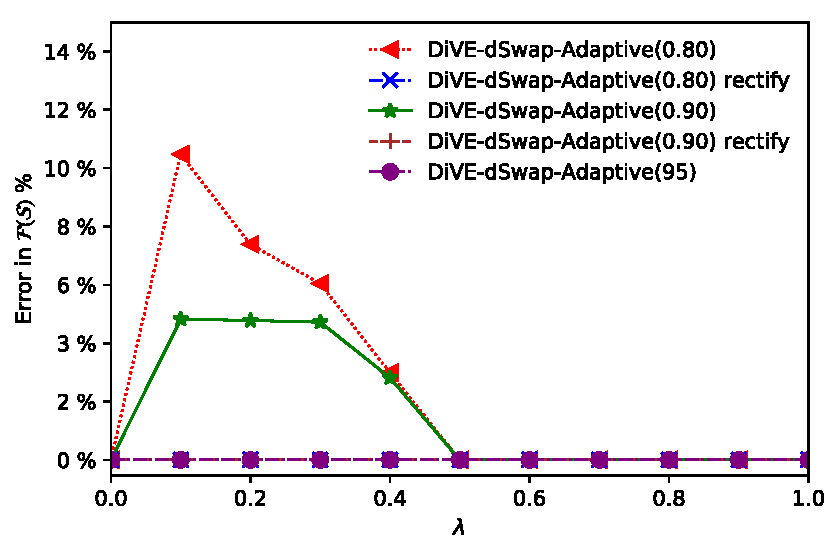
\includegraphics[width=3.0in]{figures/error_fs_rectifying_dswap}
		\caption{Error in $F(S)$ DiVE-Greedy-Adaptive and DiVE-dSwap-Adaptive after rectifying upper bound}
		\label{fig:error_fs_rectifying}
	\end{center}
\end{figure}





\begin{figure}
	\begin{center}
		\vspace{-150pt}
		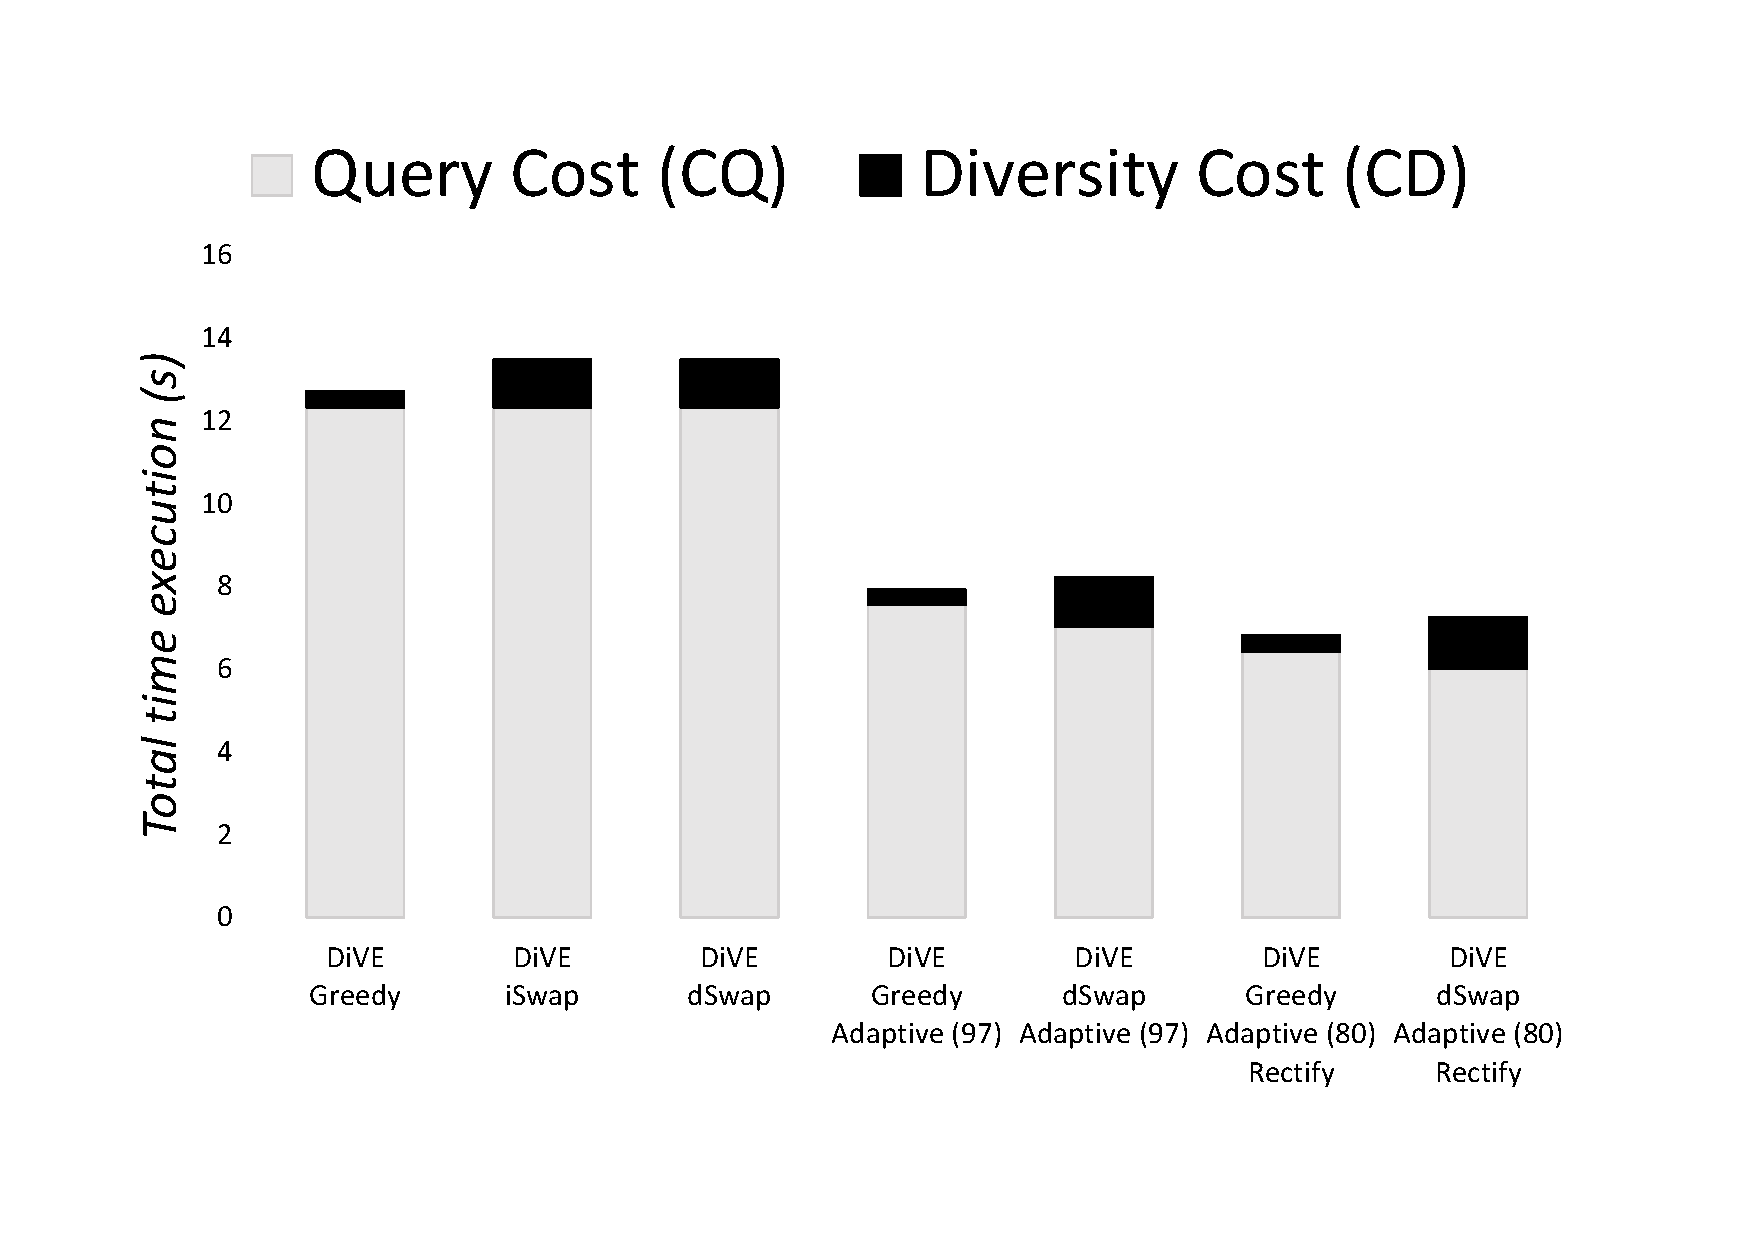
\includegraphics[width=6.5in]{figures/flight_costs_rectifying}
		%\vspace{-40pt}
		\caption{Total costs of schemes running on Flights dataset, $k = 5$, and $\lambda = 0.5$ }
		\label{fig:flight_costs_all_rectifying}
		\vspace{-10pt}
	\end{center}
\end{figure}



\begin{algorithm}
	\SetAlgoVlined
	\DontPrintSemicolon
	%This is to hide Begin keyword
	\SetKwBlock{Begin}{}{end}
	\KwIn{Set of views V and result set $S$ize k }
	\KwOut{Result set $ S \leq V $, size S = k}  
	\SetKwFunction{FgetL}{getL}
	\SetKwFunction{FgetMaxPI}{getMaxPI}
	$S \leftarrow $ two most distant views\;
	$X \leftarrow  \left[V \backslash S\right]$\;
	
	
	
	\SetKwFunction{FgetL}{getL}
	\SetKwProg{Fn}{function}{:}{}
	\Fn{\FgetL{$f$,$S$, $X$,$L$}}{
		\For{$X_i$ in set $X$}{
			\For{$S_j$ in set $S$}{
				$ d  \leftarrow setDist\left(X_i,S \right) $\;
				%$ 	X' \leftarrow [ X_i, d]$\;
				$ 	L.append([ X_i, d])$\;
			}
		}
		$ 	L \leftarrow sorted\_by\_d(L) $\;
		
		\KwRet L\;
	}
	
	%\SetKwFunction{FgetMaxPI}{getMaxPI}
	%\SetKwProg{Fn}{function}{:}{}
	%\Fn{\FgetMaxPI{$f$,$S$, $X$,$max_b$}}{
	%	$samples \leftarrow get\_samples\_PI(X)$\;
	%	$maxI\_S \leftarrow get\_maxI(S)$\;
	%	$maxI\_samples \leftarrow get\_maxI(samples)$\;
	%	
	%	\If{ $ maxI\_S > maxI $}{
	%		$ maxI \leftarrow maxI\_S$
	%	}
	%	\If{ $ maxI\_samples> maxI $}{
	%		$ maxI \leftarrow maxI\_samples$
	%	}
	%	$max_b \leftarrow maxI$		
	%	
	%	\KwRet\;
	%}
	
	%$ rectify \leftarrow False $\;
	%$ L_{base}, S_{base},S'_{base}   \leftarrow getL(S,X), S, S \cup L[X_1] $\;
	$max_b \leftarrow getMaxPI(L) $	\;
	$rectify \leftarrow False $	\;
	\;
	\While{$i < k$}{
		
		
		%	$ S' \leftarrow S $\;
		\If{$rectify = False$}{
			$ L \leftarrow getL(S,X) $\;
			$ S' \leftarrow S \cup L[X_1] $\;	
		}
		\For{$L_i$ in $L$}{
			\If{$rectify=True$}{
				$start\; loop\; at\; L[min_d]$}
			\If{ $ F\left(S'\right) < F\left(S \cup X_i, max_b\right) $}{
				$ I \leftarrow get\_I\_score(X_i) $\;
				\If{ $ F\left(S'\right) < F\left(S \cup X_i, I\right) $}{
					$ S'  \leftarrow S \cup X_i $  \;
				}
				\eIf{ $ I > max_b $}{
					$ max_b \leftarrow I $\;
					$ rectify = True $\;
					$ break (Out\ of\ Loop) $\;
				}{
					$ rectify = False $\;
					
				}
			}
			
			
			
		}
		
		%$ S  \leftarrow S'$\;
		
		
		\eIf{ $ rectify == True $}{
			%		\If{$step\_back < i - 2$}{
			%%		$ S, S' \leftarrow S_{base} $ \;
			%%	$ L \leftarrow L_{base} $ \;
			%%	$i \leftarrow  2$ \;	
			%	$ G \leftarrow fetchTempResult(i- step\_back)$\;
			%$ S, S' \leftarrow G[S], G[S'] $ \;
			%$ L \leftarrow G[L] $ \;
			%$i = i- step\_back  $\;
			%	}
			
			%			$ S, S' \leftarrow S_{base},S'_{base}  $ \;
			%			$ L \leftarrow L_{base} $ \;
			%			$i \leftarrow  2$ \;	
			
			$ G \leftarrow fetchTempResult(i- 2)$\;
			$ S, S' \leftarrow G[S], G[S'] $ \;
			$ L \leftarrow G[L] $ \;
			$i = i- 2  $\;
			
			
			
		}{
			$ storeTempResult(i, S, S', L, min_d)$\;
			$ S \leftarrow S' $ \;
			$i = i + 1  $\;
		}
		
		
		
		
		
		
		
		
		
		%
		%\If{ $ F\left(S'\right) > F\left(S\right) $}{
		%	$ S  \leftarrow S'$
		%	$  improve \leftarrow  True $\;
		%	
		%	}{
		%		$improve \leftarrow  False $\;
		%	
		%	}
	}
	$return\; S$
	\caption{\textit{DiVE} Greedy Pruning Rectifying}\label{DiVE-Greedy-Pruning-Rectifying}
\end{algorithm}


% Pruning Pseudocode

\begin{algorithm}
	\SetAlgoVlined
	\DontPrintSemicolon
	%This is to hide Begin keyword
	\SetKwBlock{Begin}{}{end}
	\KwIn{Set of views V and result set $S$ize k }
	\KwOut{Result set $ S \leq V $, size S = k}  
	\SetKwFunction{FgetL}{getL}
	$S \leftarrow $ Result set of only diversity\;
	$X \leftarrow  \left[V \backslash S\right]$\;
	
	
	
	\SetKwFunction{FgetL}{getL}
	\SetKwProg{Fn}{function}{:}{}
	\Fn{\FgetL{$f$,$S$, $X$,$L$}}{
		\For{$X_i$ in set $X$}{
			\For{$S_j$ in set $S$}{
				$ d  \leftarrow setDist\left(X_i,S \right) $\;
				%$ 	X' \leftarrow [ X_i, d]$\;
				$ 	L.append([S_j, X_i, d])$\;
			}
		}
		$ 	L \leftarrow sorted\_by\_d(L) $\;
		
		\KwRet L\;
	}
	
	%\SetKwFunction{FgetMaxPI}{getMaxPI}
	%\SetKwProg{Fn}{function}{:}{}
	%\Fn{\FgetMaxPI{$f$,$S$, $X$,$max_b$}}{
	%	$samples \leftarrow get\_samples\_PI(X)$\;
	%	$maxI\_S \leftarrow get\_maxI(S)$\;
	%	$maxI\_samples \leftarrow get\_maxI(samples)$\;
	%	
	%	\If{ $ maxI\_S > maxI $}{
	%		$ maxI \leftarrow maxI\_S$
	%	}
	%	\If{ $ maxI\_samples> maxI $}{
	%		$ maxI \leftarrow maxI\_samples$
	%	}
	%	$max_b \leftarrow maxI$		
	%	
	%	\KwRet\;
	%}
	
	$F_{current}, counter \leftarrow 0,0$\;
	$ improve, rectify \leftarrow  True, False $\;
	%$ S_{base}, L_{base}   \leftarrow S, getL(S,X) $\;
	$max_b \leftarrow getMaxPI(L) $	\;
	\;
	\While{$improve = True$}{
		$counter = counter + 1$ \;	
		\If{$rectify = False$}{
			$L \leftarrow getL(S,X)$ \;	
			$ S' \leftarrow S $\;
			
		}
		
		
		\For{$L_i$ in $L$}{
			\If{$rectify=True$}{
				$start\; loop\; at\; L[min_d]$}
			\If{ $ F\left(S'\right) < F\left(S \backslash S_j \cup X_i, max_b\right) $}{
				%	$ 	L'.append(L_i)$\;
				
				$ I \leftarrow get\_I\_score(X_i) $\;
				\If{ $ F\left(S'\right) < F\left(S\backslash S_j \cup X_i, I\right) $}{
					$ S'  \leftarrow S \backslash j \cup X_i $  \;
				}
				\eIf{ $ I > max_b $}{
					$ max_b \leftarrow I $\;
					$ rectify = True $\;
					$ break (Out\ of\ Loop) $\;
				}{
					$ rectify = False $\;
				}
			}
		}
		
		
		\eIf{$rectify == True$}{
			%			\eIf{$step\_back < counter $}{
			%	
			%					$ G \leftarrow fetchTempResult(counter - step\_back)$\;
			%				$ S, S' \leftarrow G[S], G[S'] $ \;
			%				$ L \leftarrow G[L] $ \;
			%			}{	}
			%			$ S, S' \leftarrow S_{base} $ \;
			%			$ L \leftarrow L_{base} $ \;
			%			$counter = 0$
			
			$ G \leftarrow fetchTempResult(counter=1)$\;
			$ S, S' \leftarrow G[S], G[S'] $ \;
			$ L \leftarrow G[L] $ \;
			$counter = 0 $\;
			
			$  improve \leftarrow  True $\;
			
			
		}{
			
			$ storeTempResult(counter, S, S', L, min_d)$\;
			
			\If{ $ F\left(S'\right) > F\left(S\right) $}{
				$ S  \leftarrow S'$\;
				
			}	
			
			\eIf{ $ F\left(S\right) > F_{current} $}{
				$ F_{current}  \leftarrow F\left(S\right) $\;
				$  improve \leftarrow  True $\;
				
			}{
				$improve \leftarrow  False $\;
				
			}
			
		}
		
		
		
		
		%
		%\If{ $ F\left(S'\right) > F\left(S\right) $}{
		%	$ S  \leftarrow S'$
		%	$  improve \leftarrow  True $\;
		%	
		%	}{
		%		$improve \leftarrow  False $\;
		%	
		%	}
	}
	$return\; S$
	\caption{\textit{DiVE} dSwap Pruning Rectifying}\label{DiVE-dSwap-Pruning-Rectifying}
\end{algorithm}

\end{document}



\begin{algorithm}
\SetAlgoVlined
\DontPrintSemicolon
%This is to hide Begin keyword
\SetKwBlock{Begin}{}{end}
\KwIn{Set of views V and result set $S$ize k }
\KwOut{Result set $ S \geq V $, size S = k}  
\SetKwFunction{FgetL}{getL}
\SetKwFunction{FgetMaxPI}{getMaxPI}
$S \leftarrow $ two most distant views\;
$X \leftarrow  \left[V \backslash S\right]$\;



\SetKwFunction{FgetL}{getL}
\SetKwProg{Fn}{function}{:}{}
\Fn{\FgetL{$f$,$S$, $X$,$L$}}{
	\For{$X_i$ in set $X$}{
		\For{$S_j$ in set $S$}{
			$ d  \leftarrow setDist\left(X_i,S \right) $\;
			$ 	X' \leftarrow [ X_i, d]$\;
			$ 	L.append(X')$\;
		}
	}
	$ 	L \leftarrow sorted\_by\_d(L) $\;
	
	\KwRet\;
}

\SetKwFunction{FgetMaxPI}{getMaxPI}
\SetKwProg{Fn}{function}{:}{}
\Fn{\FgetMaxPI{$f$,$S$, $X$,$max_b$}}{
	$samples \leftarrow get\_samples\_PI(X)$\;
	$maxI\_S \leftarrow get\_maxI(S)$\;
	$maxI\_samples \leftarrow get\_maxI(samples)$\;
	
	\If{ $ maxI\_S > maxI $}{
		$ maxI \leftarrow maxI\_S$
	}
	\If{ $ maxI\_samples> maxI $}{
		$ maxI \leftarrow maxI\_samples$
	}
	$max_b \leftarrow maxI$		
	
	\KwRet\;
}

$ rectify \leftarrow False $\;
$ S_{rectify}, L_{rectify}   \leftarrow S, getL(S,X) $\;
$max_b \leftarrow getMaxPI(S,X) $	\;
\;
\While{$i < k$}{
	
	
	
	
	
	
	\For{$L_i$ in $L$}{
		
		\If{ $ F\left(S'\right) < F\left(S \cup X_i, max_b\right) $}{
			$ 	L'.append(L_i)$\;
		}
		$ I \leftarrow get\_I\_score(L'_i) $\;
		\If{ $ F\left(S'\right) < F\left(S \cup X_i, I\right) $}{
			$ S'  \leftarrow S \cup X_i $  \;
		}
		\eIf{ $ I > max_b $}{
			$ max_b \leftarrow I $\;
			$ rectify = True $\;
			$ break (Out\ of\ Loop) $\;
		}{
			$ rectify = False $\;
		}
		
	}
	
	
	
	\eIf{rectify == True}{
		$ S, S' \leftarrow S_{rectify} $ \;
		$ L \leftarrow L_{rectify} $ \;
		$i \leftarrow  len(S)$ \;
		
		
	}{
		
		
		\If{ $ F\left(S'\right) > F\left(S\right) $}{
			$ S  \leftarrow S'$\;
			
		}
		$ S' \leftarrow S $\;
		$ L \leftarrow getL(S,X) $\;
		$i = i + 1  $
		
	}
	
	
	%
	%\If{ $ F\left(S'\right) > F\left(S\right) $}{
	%	$ S  \leftarrow S'$
	%	$  improve \leftarrow  True $\;
	%	
	%	}{
	%		$improve \leftarrow  False $\;
	%	
	%	}
}
$return S$
\caption{\textit{DiVE} Greedy Pruning Rectifying}\label{DiVE-Greedy-Pruning-Rectifying}
\end{algorithm}


% Pruning Pseudocode

\begin{algorithm}
\SetAlgoVlined
\DontPrintSemicolon
%This is to hide Begin keyword
\SetKwBlock{Begin}{}{end}
\KwIn{Set of views V and result set $S$ize k }
\KwOut{Result set $ S \geq V $, size S = k}  
\SetKwFunction{FgetL}{getL}
$S \leftarrow $ Result set of only diversity\;
$X \leftarrow  \left[V \backslash S\right]$\;



\SetKwFunction{FgetL}{getL}
\SetKwProg{Fn}{function}{:}{}
\Fn{\FgetL{$f$,$S$, $X$,$L$}}{
	\For{$X_i$ in set $X$}{
		\For{$S_j$ in set $S$}{
			$ d  \leftarrow setDist\left(X_i,S \backslash S_j\right) $\;
			$ 	X' \leftarrow [S_j, X_i, d]$\;
			$ 	L.append(X')$\;
		}
	}
	$ 	L \leftarrow sorted\_by\_d(L) $\;
	
	\KwRet\;
}

\SetKwFunction{FgetMaxPI}{getMaxPI}
\SetKwProg{Fn}{function}{:}{}
\Fn{\FgetMaxPI{$f$,$S$, $X$,$max_b$}}{
	$samples \leftarrow get\_samples\_PI(X)$\;
	$maxI\_S \leftarrow get\_maxI(S)$\;
	$maxI\_samples \leftarrow get\_maxI(samples)$\;
	
	\If{ $ maxI\_S > maxI $}{
		$ maxI \leftarrow maxI\_S$
	}
	\If{ $ maxI\_samples> maxI $}{
		$ maxI \leftarrow maxI\_samples$
	}
	$max_b \leftarrow maxI$		
	
	\KwRet\;
}


$ F_{current}, improve, rectify \leftarrow  0, True, False $\;
$ S_{rectify}, L_{rectify}   \leftarrow S, getL(S,X) $\;
$max_b \leftarrow getMaxPI(S,X) $	\;
\;
\While{improve = True}{
	
	
	\For{$L_i$ in $L$}{
		
		\If{ $ F\left(S'\right) < F\left(S \backslash S_j \cup X_i, max_b\right) $}{
			$ 	L'.append(L_i)$\;
		}
		$ I \leftarrow get\_I\_score(L'_i) $\;
		\If{ $ F\left(S'\right) < F\left(S\backslash S_j \cup X_i, I\right) $}{
			$ S'  \leftarrow S \backslash j \cup X_i $  \;
		}
		\eIf{ $ I > max_b $}{
			$ max_b \leftarrow I $\;
			$ rectify = True $\;
			$ break (Out\ of\ Loop) $\;
		}{
			$ rectify = False $\;
		}
		
	}
	
	
	
	\eIf{rectify == True}{
		$ S, S' \leftarrow S_{rectify} $ \;
		$ L \leftarrow L_{rectify} $ \;
		$improve \leftarrow  True$ \;
		
		
	}{
		
		
		\If{ $ F\left(S'\right) > F\left(S\right) $}{
			$ S  \leftarrow S'$\;
			
		}
		
		\eIf{ $ F\left(S\right) > F_{current} $}{
			$ F_{current}  \leftarrow F\left(S\right) $\;
			$  improve \leftarrow  True $\;
			
		}{
			$improve \leftarrow  False $\;
			
		}
		$ S' \leftarrow S $\;
		$ L \leftarrow getL(S,X) $\;
		
	}
	
	%
	%\If{ $ F\left(S'\right) > F\left(S\right) $}{
	%	$ S  \leftarrow S'$
	%	$  improve \leftarrow  True $\;
	%	
	%	}{
	%		$improve \leftarrow  False $\;
	%	
	%	}
}
$return S$
\caption{\textit{DiVE} dSwap Pruning Rectifying}\label{DiVE-dSwap-Pruning-Rectifying}
\end{algorithm}


% Pruning Pseudocode

\begin{algorithm}
\SetAlgoVlined
%This is to hide Begin keyword
\SetKwBlock{Begin}{}{end}
\KwIn{Set of views V and result set $S$ize k }
\KwOut{Result set $ S \geq V $, size S = k}  
$S \leftarrow $ Result set of only diversity\;
$X \leftarrow  \left[V \backslash S\right]$\;
$F_{current} \leftarrow 0 $\;
$  improve \leftarrow  True $\;
$ max_b  \leftarrow\sqrt{2} $\;
%$ S_{rectify}  \leftarrow [] $\;
%$ X_{rectify}  \leftarrow [] $\;
\While{improve = True}{
	%$ X' \leftarrow [] $\;
	\For{$X_i$ in set $X$}{
		\For{$S_j$ in set $S$}{
			$ d  \leftarrow setDist\left(X_i,S \backslash S_j\right) $\;
			$ 	newX \leftarrow [S_j, X_i, d]$\;
			$ 	X'.append(newX)$\;
		}
	}
	$ 	X' \leftarrow sorted\_by\_d(X') $\;
	$ S' \leftarrow S $\;
	$ rectify  = False $\;
	\eIf{ $ max_b == \sqrt{2} $}{
		\For{$i$ in set $X'$}{
			
			\If{ $ F\left(S'\right) < F\left(S \backslash X'[i][0] \cup X'[i][1], max_b\right) $}{
				$ 	X''.append(X'[i][1])$\;
			}
		}
		
		$n \leftarrow pi - len(S)$\;
		$samples \leftarrow X''[0\colon n]$\;
		$maxI\_S \leftarrow get\_maxI(S)$\;
		$maxI\_samples \leftarrow get\_maxI(samples)$\;
		
		\If{ $ maxI\_S > maxI $}{
			$ maxI \leftarrow maxI\_S$
		}
		\If{ $ maxI\_samples> maxI $}{
			$ maxI \leftarrow maxI\_samples$
		}
		$max\_b \leftarrow maxI$	
		
		\For{$i$ in set $X''$}{
			\For{$j$ in set $S$}{
				\If{ $ F\left(S'\right) < F\left(S \backslash S_j \cup X''[i], max_b\right)  $}{
					$ 	X'''.append(X''[i])$\;
					
				}
				$ I \leftarrow get\_I\_score(X'''[i]) $\;
				\If{ $ F\left(S'\right) < F\left(S \backslash S_j \cup X'''[i], I\right) $}{
					$ S'  \leftarrow S \backslash j \cup X'''[i] $  \;
				}
				\If{ $ I > max_b $}{
					$ max_b \leftarrow I $\;
					$ rectify = True $\;
					$ break (Out\ of\ Loop) $\;
				}
			}
		}
		
	}{ 
		
		
	}
	%
	%\If{ $ F\left(S'\right) > F\left(S\right) $}{
	%	$ S  \leftarrow S'$
	%	$  improve \leftarrow  True $\;
	%	
	%	}{
	%		$improve \leftarrow  False $\;
	%	
	%	}
}
%return S
\caption{\textit{DiVE} dSwap Pruning Rectifying}\label{DiVE-dSwap-Pruning-Rectifying}
\end{algorithm}

\begin{algorithm}
\LinesNumbered
\setcounter{AlgoLine}{37}
% This is to restore vline mode if you did not take the package as \usepackage[linesnumbered,ruled,vlined]{algorithm2e}
\SetAlgoVlined
%This is to hide Begin keyword
\SetKwBlock{Begin}{}{end}
\Begin{
	\eIf{...}{...}
	{
		
		\For{$X_i$ in set $X'$}{
			\If{ $ F\left(S'\right) < F\left(S \backslash X'[i][0] \cup X'[i][1], max_b\right) $}{
				$ 	X''.append(X'[i][1])$\;
			}
			$ I \leftarrow get\_I\_(X''[i]) $\;
			\If{ $ F\left(S'\right) < F\left(S \backslash S_j \cup X''[i], I\right) $}{
				$ S'  \leftarrow S \backslash j \cup X''[i] $  \;
			}
			\If{ $ I > max\_b $}{
				$ max\_b \leftarrow I $ \;
				$ rectify = True $\;
				$ break (Out\ of\ Loop) $\;
			}
			
		}
		
	}
	
	\eIf{rectify == True}{
		$improve \leftarrow  True$ \;
		
		
	}{
		
		
		\If{ $ F\left(S'\right) > F\left(S\right) $}{
			$ S  \leftarrow S'$\;
			
		}
		
		\eIf{ $ F\left(S\right) > F_{current} $}{
			$ F_{current}  \leftarrow F\left(S\right) $\;
			$  improve \leftarrow  True $\;
			
		}{
			$improve \leftarrow  False $\;
			
		}
		
	}
	
}   
$return S$ 
\end{algorithm}


\SetKwFunction{FgetNewS}{getNewS}
\SetKwProg{Fn}{function}{:}{}
\Fn{\FgetNewS{$f$,$S$, $X$,$max_b$, $G$}}{
$ S' \leftarrow S $\;
\For{$L_i$ in $L$}{
	
	\If{ $ F\left(S'\right) < F\left(S \cup X_i, max_b\right) $}{
		$ I \leftarrow get\_I\_score(X_i) $\;
		\If{ $ F\left(S'\right) < F\left(S \cup X_i, I\right) $}{
			$ S'  \leftarrow S \cup X_i $  \;
		}
		\eIf{ $ I > max_b $}{
			$ max_b \leftarrow I $\;
			$ rectify = True $\;
			$ break (Out\ of\ Loop) $\;
		}{
			$ rectify = False $\;
			
		}
		
		
	}
	
	
}
\If{ $ F\left(S'\right) > F\left(S\right) $}{
	$ S  \leftarrow S'$\;
}
$ G  \leftarrow S, rectify $\;
\KwRet G\;
}


%\section{Proposed algorithm's Figure}
%We proposed DiVE scheme using two kinds of popular heuristic approach which are Greedy and Swap techniques. Figure \ref{fig:algorithm-figure} shows our proposed scheme technique. In case of Greedy, the set $ S $ is initialized by two most distant views. In each iteration, the best view in $ X $ that can maximize objective function $F(S)$ will be added to the set $ S $. Meanwhile, for the Swap case, the set $ S $ is initialized by the most diverse $  k $ views and in each iteration, all candidates views in $ X $ will be interchanged to set $ S $ and view which can improve the current objective function $F(S)$ will replace a view in set $ S $.
%
%The $setDist$ score is used to sort all candidate views in $ X $, the highest score means that views is more diverse to set $ S $. The current bound is utilized to compute the estimate utility of each candidate view. First, the theoritical upper bound ($ \sqrt{2} $) is used and this bound is updated while the actual importace score of view has been known. To avoid the wrong current bound, samping based on prediction interval is used. Before running the program, user needs to defined what PI that she wants to use. For instance, while users set PI to 80 then after 9 views is executed the current bound will be updated to the upper bound which have seen so far. The most used PI can be defined as following: 
%
%\begin{itemize}[noitemsep]
%	\item PI80: need to execute 9 views
%	\item PI85: need to execute 12 views
%	\item PI90: need to executes 20 views
%	\item PI95: need to executes 40 views
%	\item PI97: need to executes 60 views
%\end{itemize}
%
%
%\begin{figure}
%	\begin{center}
%		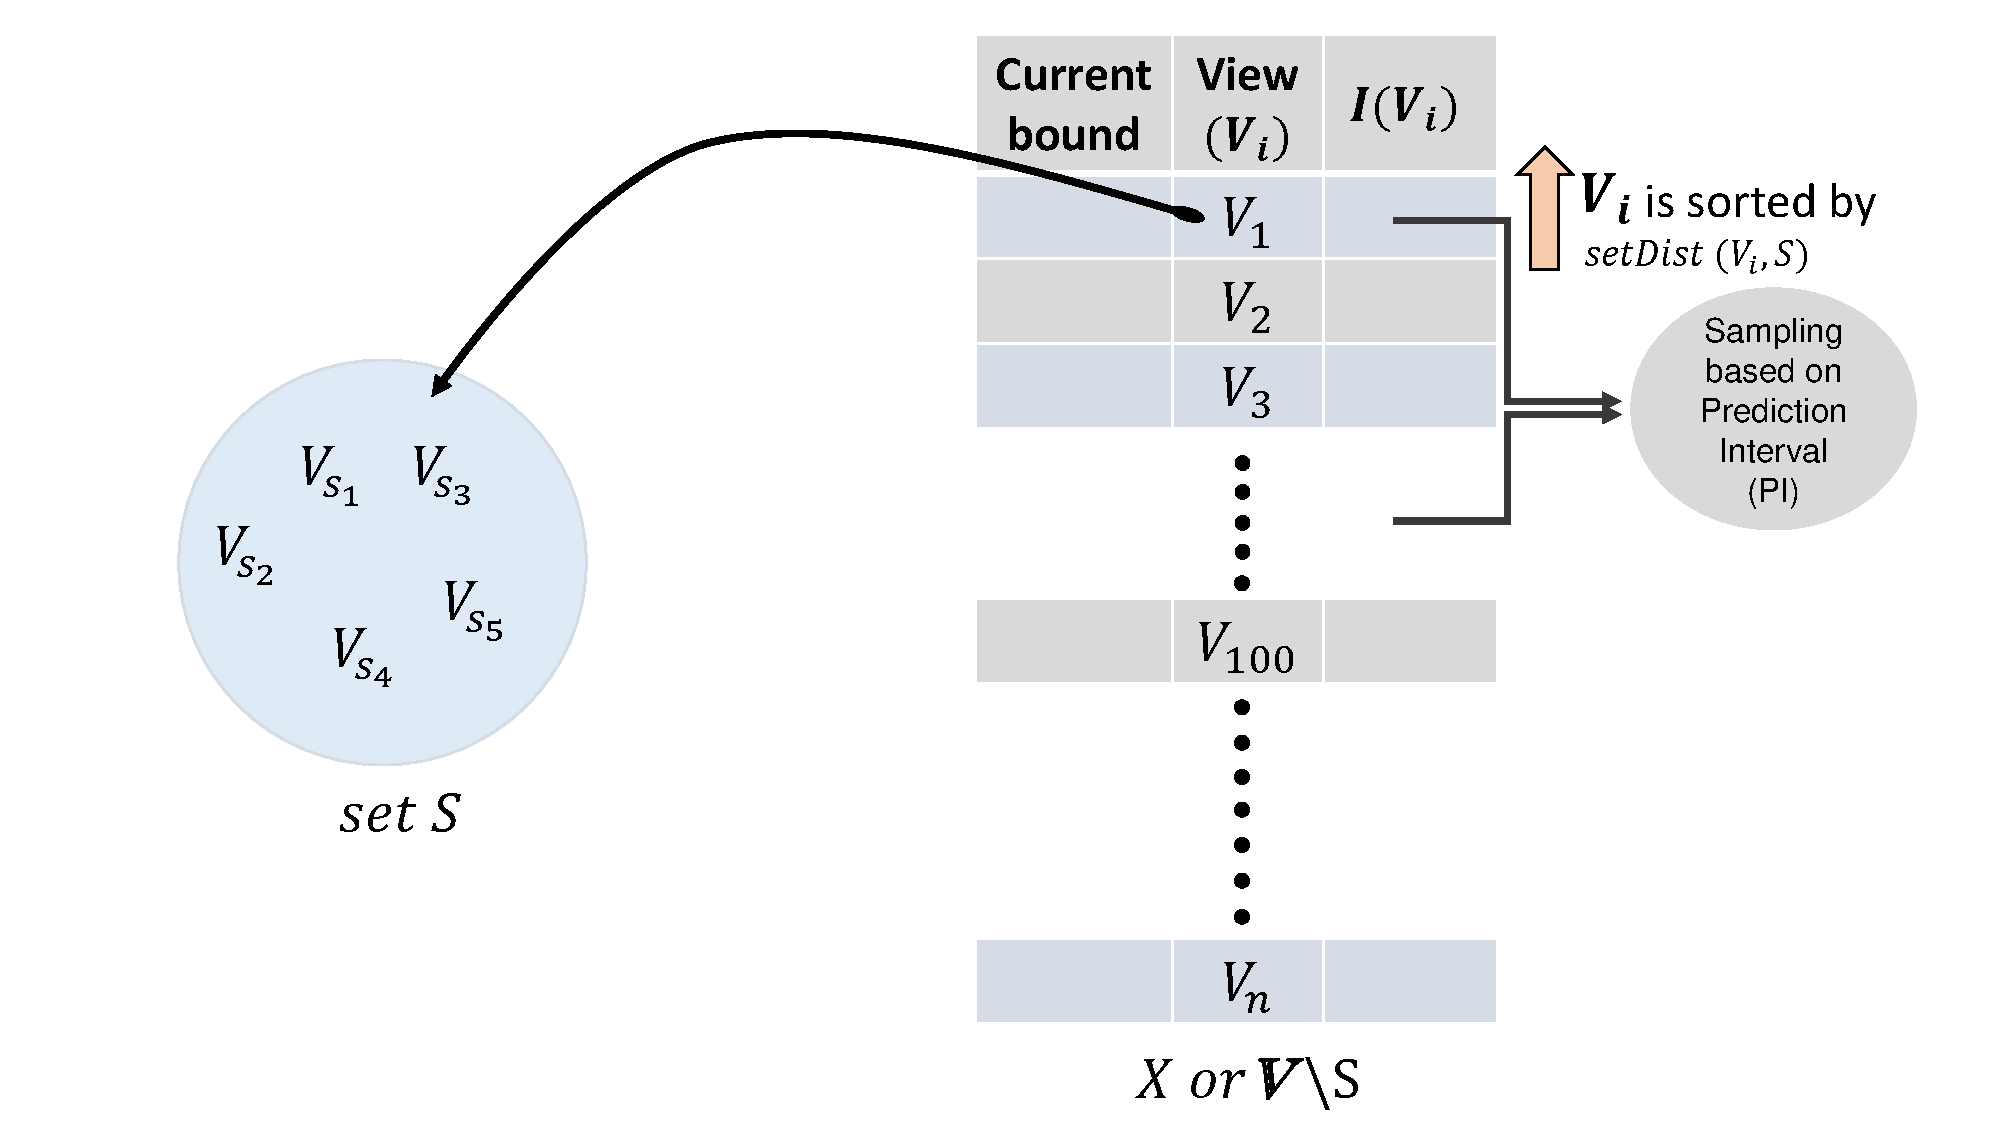
\includegraphics[width=5.0in]{figures/Algorithm}
%		\vspace{-12pt}
%		\caption{Utilizing $setDist$ score to sort candidate views and update current upper bound to optimize the pruning performance}
%		\label{fig:algorithm-figure}
%		
%	\end{center}
%\end{figure}


%For the general case, Euclidean distance $d$ is defined as following: 
%$d = \sum{(x-y)^2} = \sum x^2 + \sum y^2 - 2\sum xy$. Given that in probability vectors all values are nonnegative, $d$ is max when the last term is zero, then $d = \sum x^2 + \sum y^2$.
%
%All values are between 0 and 1 (sum up to 1), $\sum x = \sum y = 1$. In such a vector, its theoretical maximum is attained when all its entries are 0 except one which is 1, it is when $\sum x^2 = \sum x$ and $\sum y^2 = \sum y$. It also follows from the above description, that then $\sum xy$ can very easily happen to be zero (since in each vector there is just single nonzero element).
%\newline

%Example maximum condition for two bins case: 
%\newline
%
%$\sum a = \sum b = 1$, $a , b \geq 0$
%\newline
%
%$(\sum a)^2 + (\sum b)^2 \geq \sum a^2 + \sum b^2$
%\newline
%
%$(\sum a)^2 + (\sum b)^2 \geq \sum a^2 + \sum b^2 - \sum 2ab $ 
%\newline
%
%$(\sum a)^2 + (\sum b)^2 \geq \sum (a^2 +  b^2 -  2ab)  $ 
%\newline
%
%$(\sum a)^2 + (\sum b)^2 \geq \sum (a-b)^2  $ 
%\newline
%
%$1 + 1 \geq \sum (a-b)^2  $ 
%\newline
%
%$\sqrt{2} \geq \sqrt{\sum (a-b)^2}  $ 
%\newline

%Max-sum is bi-criteria objective function to maximize the sum of the relevance and dissimilarity of the selected set, which can be defined as follows:
%
%\begin{equation}
%F\left(S\right) =  \left(1-\lambda\right) * I\left(S\right) + \lambda * f\left(S,D\right)
%\label{objectif_function}
%\end{equation}
%
%Where, 
%$ I\left(S\right)= \sum_{i=1}^{k} \dfrac{I(V_i )}{I_u}, V_i  \in S $ and $ f\left(S,D\right)= \dfrac{1}{k\left(k-1\right)}  \sum_{i=1}^{k} \sum_{j>i}^{k} D\left(V_i,V_j\right) ,V_i,V_j  \in S $
%\newline
%
%Meanwhile, Max-min diversification is the bi-criteria objective function that maximize the \textit{minimum} relevance and dissimilarity of the selected set. Based on the work of Gollapudi (An axiometic approach for result diversificaiton), this objective function can be defined as follows: 
%
%\begin{equation}
%F\left(S\right) = (1-\lambda) * \underset{u \in S} {\mathrm{min}} \ w\left(u\right)  + \lambda * \underset{u,v \in S} {\mathrm{min}} d\left(u,v\right)
%\end{equation}
%
%While Max-min diversification is to maximize the minimum of importance score, I am not sure this approach is relevant or not for our work. 